\setAuthor{Jaan Kalda}
\setRound{lahtine}
\setYear{2021}
\setNumber{G 4}
\setDifficulty{4}
\setTopic{TODO}

\prob{Kuiv õhk}
Talvel võib liigne kuivus toas probleeme tekitada: alla 20-protsendine suhteline niiskus ei mõju hästi inimese nahale ja limaskestadele. Eeldage, et välisõhk siseneb tuppa läbi ventilatsiooni ja toaõhk vahetub väljast tulnud õhuga ühe tunni jooksul peaaegu täielikult ning et toas hoitakse 20-kraadilist õhutemperatuuri. Millise välisõhu temperatuuri juures langeb toas suhteline niiskus alla 20\%, kui väljas on suhteline niiskus 80\%? Küllastunud auru rõhu sõltuvus temperatuurist on toodud graafikul.\\
\emph{Märkus:} suhteliseks niiskuseks nimetatakse õhus oleva veeauru osarõhu ja antud temperatuuri juures küllastunud veeauru osarõhu suhet.

\begin{figure}[h]
  \vspace{-1em}
  \centering
  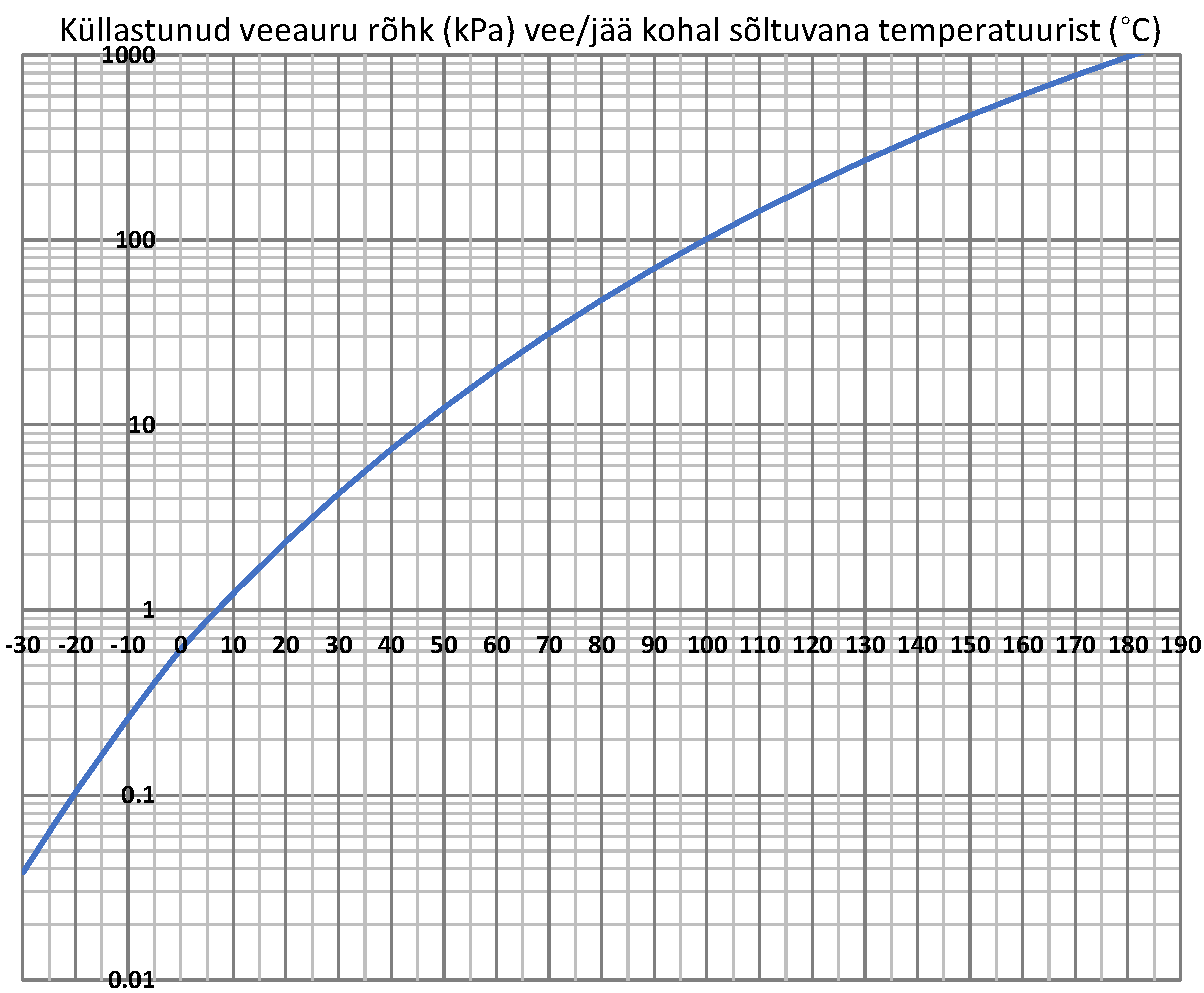
\includegraphics[width=0.95\textwidth]{2021-lahg-04-yl.pdf}
  \vspace{-1em}
\end{figure}


\hint

\solu
Kui õhk siseneb ruumi, siis vee moolide suhe kogu gaasi moolide arvu ei muutu, olgu need teatud koguse tuppa siseneva õhu jaoks vastavalt $\nu_v$ ja $\nu_k$. Ideaalse gaasi olekuvõrrandist saame vee osarõhu ja kogu rõhu jaoks vastavalt $p_vV=\nu_vRT$ ja $p_kV=\nu_kRT$, millest $p_v = p_k\frac{\nu_v}{\nu_k}$. Arvestades, et kogurõhk on nii toas kui väljas võrdne atmosfäärirõhuga $p_0$, saame suhtelise niiskuse jaoks avaldise $r=\frac{p_v}{p(T)}=\frac{p_0}{p(T)}\frac{\nu_v}{\nu_k}$, kus $p(T)$ tähistab küllastunud auru rõhku sõltuvuses temperatuurist ja on leitav graafikult. Tähistagu $r_v=\frac{p_0}{p(T_v)}\frac{\nu_v}{\nu_k}$ ja $r_s=\frac{p_0}{p(T_s)}\frac{\nu_v}{\nu_k}$ vastavalt suhtelisi niiskusi väljas ja sees. Seega $p(T_v)=p(T_s)\frac{r_s}{r_v}=\frac{p(T_s)}{4}$; graafikult loeme, et $p(T_s)\approx \SI{2,2}{kPa}$ (NB! tüvenumbrite lugemisel tuleb meeles pidada, et tegemist on logaritmilise graafikuga!) ning seega $p(T_v)\approx\SI{550}{Pa}$. Graafikult leiame ka sellele rõhule vastava temperatuuri, $T_v \approx \SI{-1}\celsius$.
\probend